\documentclass[10pt,a4paper]{article}
\usepackage[utf8]{inputenc}
\usepackage[ngerman]{babel}
\usepackage{amsmath}
\usepackage{amsfonts}
\usepackage{amssymb}
\usepackage{graphicx}
\usepackage{natbib}
\usepackage{float}
\usepackage{hyperref}
\usepackage{acronym}
\author{\makebox[.9\textwidth]{Sebastian Knigge, BSc BSc}\\ Universität Wien \and \textit{Betreuer} \\ Dipl.-Ing. Martin Glanzer \\Department of Statistics and Operations Research\\ Universität Wien }
\title{SEMINARARBEIT\\[3mm] \normalsize{Kurs: 040774 PR}}



\begin{document}

\maketitle

\newpage

\tableofcontents

\section*{Abkürzungsverzeichnis}
\begin{acronym}[m.a.W....]
  \acro{D.h.}{das heißt}
 \acro{LSM}{Least Squares Monte Carlo}
 \acro{bspw.}{bespielsweise}
 \acro{m.a.W.}{mit anderen Worten}
 \acro{s.}{siehe}
 \acro{sog.}{sogenannt/e/s}
 \acro{vgl.}{vergleiche}
 \acro{ZP}{Zeitpunkt}
\end{acronym}

\newpage

\section{Theoretische Grundlagen und Hintergr"unde}

\subsection{Optionen und ihre Bewertung}
Diese Arbeit behandelt die Bewertung von Optionen - im Speziellen amerikanische Put Optionen.
Dem Leser soll aber zunächst ein Überblick über die verschiedenen Arten von Optionen und deren Wesen verschafft werden.\\
Hans Becker beschreibt in \glqq Investitionen und Finanzierung \grqq Optionen als \glqq bedingte Termingeschäfte \grqq \cite[S.313]{Becker2012} weil eine Option im Gegensatz zu einem Forward oder Future für den Käufer des Finanztitels nur ein Recht, aber keine Pflicht auf Ausübung des Geschäftes einräumt. Ein Käufer hält eine Position in der \textit{long position}  ein Verkäufer in der \textit{short position}. Klarerweise ist - je nach dem um welche Partei es sich handelt -  die Auszahlung der Option unterschiedlich.\\
Weiters gibt es zwei Grundtypen von Optionen. Kaufoptionen, sog. \textit{calls} und Verkaufsoptionen, sog. \textit{puts}. Weitere wichtige Begriffe im Zusammenhang mit Optionen sind der Basiswert oder das \glqq underlying", also der zugrundeliegende Stock (Aktie), im Falle einer Aktienoption, und der Basispreis oder auch \textit{strike price}. Für eine \glqq europäische"\ Verkaufsoption bspw. hat der Käufer das Recht das underlying zu 
einem festgelegten Zeitpunkt (sog. \textit{maturity}) und zu einem festgelegten Preis zu verkaufen, für den Verk"aufer, der die Option in short position hält, besteht die Pflicht das Basisprodukt zu diesem Zeitpunkt zu kaufen, falls die Option vom Käufer ausgeführt wird.\\
Es gibt eine weitere Unterscheidung von Optionen hinsichtlich des Ausübungs-zeitpunktes. Man unterscheidet in \glqq europäische\grqq und \glqq amerikanische"\ Optionen. Europäische Optionen dürfen ausschließlich zum \textit{expiration date} ausge"ubt werden, wohingegen amerikanische Optionen zu jedem Zeitpunkt bis zum \textit{expiration date}  ausge"ubt werden können (vgl.\cite{Hull}, S.7).\\
Für eine amerikanische put Option kann im Aus"ubungszeitpunkt, der vorher freilich nicht bekannt ist, die Auszahlung wie im folgenden Plot gezeichnet werden (s. Abbildung \ref{fig:PlotOption}).

\begin{figure}[H]
  \centering
  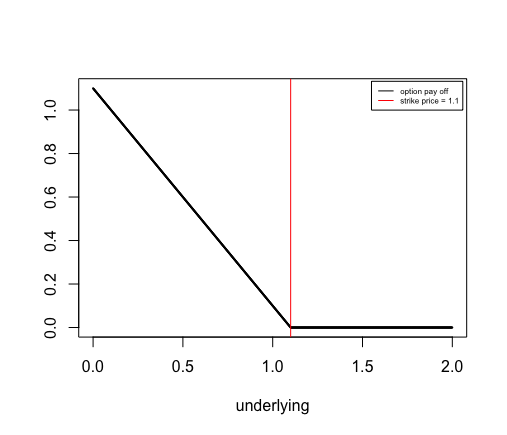
\includegraphics[scale=0.7]{PlotOption.png}
  \label{fig:PlotOption}
  \caption{Auszahlung einer Put Option mit strike 1.1}
\end{figure}

Für eine europäische Option, bei welcher der Ausübungszeitpunkt bekannt ist, ist die Bewertung der Option im Black-Scholes Moell in geschlossener Form möglich. Diese ist in \cite{Hull} auf S.313 zu finden. Weiters führt Hull auch eine Skizze zur Herleitung an.\\
Die Schwierigkeit bei der Bewertung amerikanischer Optionen besteht darin, dass der Ausübungszeitpunkt nicht bekannt ist. Der K"aufer der Option muss also zu jedem Zeitpunkt abwägen, ob die Option ausgeübt werden soll, oder ob die Alternative d.h. die Beibehaltung der Option und eine spätere Aus"ubung sinvoller ist. 
Der Lonstaff Schwartz Algorithmus besteht im Wesentlichen aus zwei Teilen. Zum einen, der grundlegenden Simulation von einer ausreichenden Zahl an Preis Trajektorien des \textit{underlying} über die Zeit. Und dem Algorithmus selbst wobei iterativ zu jedem Zeitpunkt der Auszahlungsbetrag bei Aus"ubung und der Erwartungswert bei Beibehaltung verglichen wird. Dieser Erwartungswert berechnet sich durch Schätzen eines linearen Modells der \textit{stock} prices auf die ex-post Auszahlungen mittels kleinste Quadrate Methode. Davon is auch der Name  Least Squares Monte Carlo (LSM) des Algorithmus abgeleitet.\footnote{vgl. \cite[S.114]{schwartz2001}} 


\subsection{Illustratives Beispiel}

Folgendes Beispiel soll helfen den Least Squares Monte Carlo (LSM) Algorithmus zu veranschaulichen. 

Um die Bewertung amerikanischer Optionen zu veranschaulichen, ist es sinnvoll, zunächst sog. \glqq Bermuda Optionen\grqq zu betrachten. Dieser Typ von Optionen, lässt eine Ausübung am Laufzeitende, wie bei der europäischen Option zu, als auch an festgelegten Ausübungszeitpunkten über die Laufzeit hinweg (z.B. zum Monatsende oder Jahresende). Weil dieser Optionstyp sowohl Charakteristika einer europäischen Option als auch einer amerikanischen Option hinsichtlich der Ausübung vereint, nennt man sie auch „Bermuda-Optionen“. \footnote{\textit{Bermuda} bezieht sich auf die geographische Lage der Bermuda Inseln zwischen Amerika und Europa}\footnote{vgl. \cite{Fries}}

Der aktuelle Preis sei normiert und liegt bei 1. Der Strike Preis (i.e. Aus"ubungspreis der Option) bei $K=1.1$. Man gehe weiters davon aus, dass die Option j"ahrlich ausge"ubt werden kann und eine Laufzeit von 4 Jahren hat.\\
Im ersten Schritt werden sog. Pfade simuliert. Hierbei handelt es sich um den Preis des Underlyings. Die Anzahl der Pfade ist dabei beliebig.\footnote{Wie bei Monte-Carlo simulationen "ublich, betimmt allerdings die Zahl der Simulationen die Robustheit der Schätzung} Um das Beispiel "ubersichtlich zu gestalten, werden wir hier nur 10 Pfade simulieren. Jeder Pfad (notiert als Vektor mit 5 Elementen), besteht aus dem konstanten Startpreis (zum ZP $t=0$) und 4 simulierten Preisen.\\


Tabelle \ref{tab:M} zeigt die Matrix der Simulationen des Underlyings. Ein Plot der Pfade findet sich in Abbildung \ref{fig:pfade}.





\begin{table}[H] \centering 
  \caption{Simulationsmatrix} 
  \label{tab:M} 
\begin{tabular}{@{\extracolsep{5pt}} cccccc} 
\\[-1.8ex]\hline 
\hline \\[-1.8ex] 
 & t0 & t1 & t2 & t3 & t4 \\ 
\hline \\[-1.8ex] 
1 & $1$ & $0.832$ & $1.199$ & $0.879$ & $1.007$ \\ 
2 & $1$ & $0.931$ & $1.039$ & $0.973$ & $0.885$ \\ 
3 & $1$ & $1.091$ & $1.588$ & $1.280$ & $1.549$ \\ 
4 & $1$ & $1.021$ & $1.054$ & $0.836$ & $1.099$ \\ 
5 & $1$ & $1.039$ & $0.872$ & $0.685$ & $0.931$ \\ 
6 & $1$ & $1.515$ & $2.051$ & $1.545$ & $1.751$ \\ 
7 & $1$ & $1.138$ & $1.288$ & $1.539$ & $1.705$ \\ 
8 & $1$ & $0.620$ & $0.030$ & $0.077$ & $0.058$ \\ 
9 & $1$ & $0.794$ & $1.004$ & $0.663$ & $0.571$ \\ 
10 & $1$ & $0.866$ & $0.724$ & $1.101$ & $0.986$ \\ 
\hline \\[-1.8ex] 
\end{tabular} 
\end{table} 


\begin{figure}[H]








































